

\documentclass{report}
\usepackage[utf8]{inputenc}

\usepackage[letterpaper, total={6in, 8in}]{geometry}
\usepackage{graphicx}
\usepackage{listings}
\usepackage{esint}

\newcommand{\unitx}{\mathbf{\hat{x}}}
\newcommand{\unity}{\mathbf{\hat{y}}}
\newcommand{\unitz}{\mathbf{\hat{z}}}
\newcommand{\unitr}{\mathbf{\hat{r}}}
\newcommand{\unittheta}{\boldsymbol{\hat{\theta}}}
\newcommand{\unitphi}{\boldsymbol{\hat{\phi}}}


\title{Electrodynamics}
\author{Hongyu Zhang}
\date{\today}



\usepackage{amsmath}
%%% Uncomment one at a time
% \usepackage{newtxtext,newtxmath}
% \usepackage{tgtermes}\usepackage[lite]{mtpro2}
% \usepackage{stix}
% \usepackage{mathptmx}

\newcommand{\vect}[1]{\mathbf{#1}}


\begin{document}
\maketitle
\renewcommand\thesection{1.\arabic{section}}
\setcounter{section}{0}
\renewcommand\theequation{1.\arabic{equation}}
\setcounter{equation}{0}
\newcommand{\Problem}{{\bf Problem: }}





\chapter{All the Math + Notation}
\section{Vector Derivatives}

\textbf{Cartesian.} $\displaystyle d\mathbf{l} = dx \mathbf{\hat{x}} + dy \mathbf{\hat{y}} + dz \mathbf{\hat{z}}$; $d\tau = dxdydz$.

\noindent Gradient: $\displaystyle \nabla t = \frac{\partial t}{\partial x}\unitx  + \frac{\partial t}{\partial y}\unity + \frac{\partial t}{\partial z}\unitz$

\noindent Divergence:  $\displaystyle \nabla \cdot \mathbf{v} = \frac{\partial v_x}{\partial x}  + \frac{\partial v_y}{\partial y} + \frac{\partial v_z}{\partial z}$

\noindent Curl: $\displaystyle \nabla \times \mathbf{v} = \frac{\partial v_z}{\partial y} - \frac{\partial v_y}{\partial z}\unitx  + \left( \frac{\partial v_x}{\partial z} - \frac{\partial v_z}{\partial x} \right)\unity + \left( \frac{\partial v_y}{\partial x} - \frac{\partial v_x}{\partial y} \right)\unitz$

\noindent Laplacian: $\displaystyle \nabla^2 t = \frac{\partial^2 t}{\partial x^2}  + \frac{\partial^2 t}{\partial y^2} + \frac{\partial^2 t}{\partial z^2}$


\vspace{1em}
\noindent \textbf{Spherical.} $\displaystyle d\mathbf{l} = dr \mathbf{\hat{r}} + r d\theta \boldsymbol{\hat{\theta}} + r \sin{\theta} d\phi \boldsymbol{\hat{\phi}}$; $d\tau = r^2 \sin{\theta} drd\theta d\phi$.

\noindent Gradient: $\displaystyle \nabla t = \frac{\partial t}{\partial x}\unitx  + \frac{\partial t}{\partial y}\unity + \frac{\partial t}{\partial z}\unitz$

\noindent Divergence:  $\displaystyle \nabla \cdot \mathbf{v} = \frac{\partial v_x}{\partial x}  + \frac{\partial v_y}{\partial y} + \frac{\partial v_z}{\partial z}$

\noindent Curl: $\displaystyle \nabla \times \mathbf{v} = \frac{\partial v_z}{\partial y} - \frac{\partial v_y}{\partial z}\unitx  + \left( \frac{\partial v_x}{\partial z} - \frac{\partial v_z}{\partial x} \right)\unity + \left( \frac{\partial v_y}{\partial x} - \frac{\partial v_x}{\partial y} \right)\unitz$

\noindent Laplacian: $\displaystyle \nabla^2 t = \frac{\partial^2 t}{\partial x^2}  + \frac{\partial^2 t}{\partial y^2} + \frac{\partial^2 t}{\partial z^2}$


\section{Dirac Delta Function}
\subsection{One-Dimentional Dirac Delta Function}
\begin{equation}
    \int_{-\infty}^\infty f(x)\delta(x-a) dx = f(x)
\end{equation}
\subsection{The Three-Dimentional Delta Function}
\begin{equation}
    \int_{\mathrm{all space}} f(\mathbf{r})\delta^3(\mathbf{r} - \mathbf{a})d\tau = f(\mathbf{a})
\end{equation}


\noindent \textbf{Using Dirac Delta function to solve paradox when applying divergence theorem to a point charge:}


\noindent Setup: 
\begin{equation}
    \mathbf{v} = \frac{1}{r^2} \mathbf{\hat{r}}.
\end{equation}

\begin{equation}
    \int \nabla \cdot \mathbf{v} d \tau = \int 0 d \tau = 0,
\end{equation}
except at the origin where the $\mathbf{v}$ blows up! (So, it really should be $4\pi$.) And 
\begin{equation}
    \oint \mathbf{v} \cdot d\mathbf{a} = 4 \pi \neq  \int \nabla \cdot \mathbf{v} d \tau.
\end{equation}
Resolution: for the point charge: 
\begin{equation}
    \nabla \cdot \left( \frac{\mathbf{\hat{r}}}{r^2} \right) = 4\pi \delta^3(\mathbf{r}).
\end{equation}

\section{Notation}
\begin{figure}[h!]
    \centering
    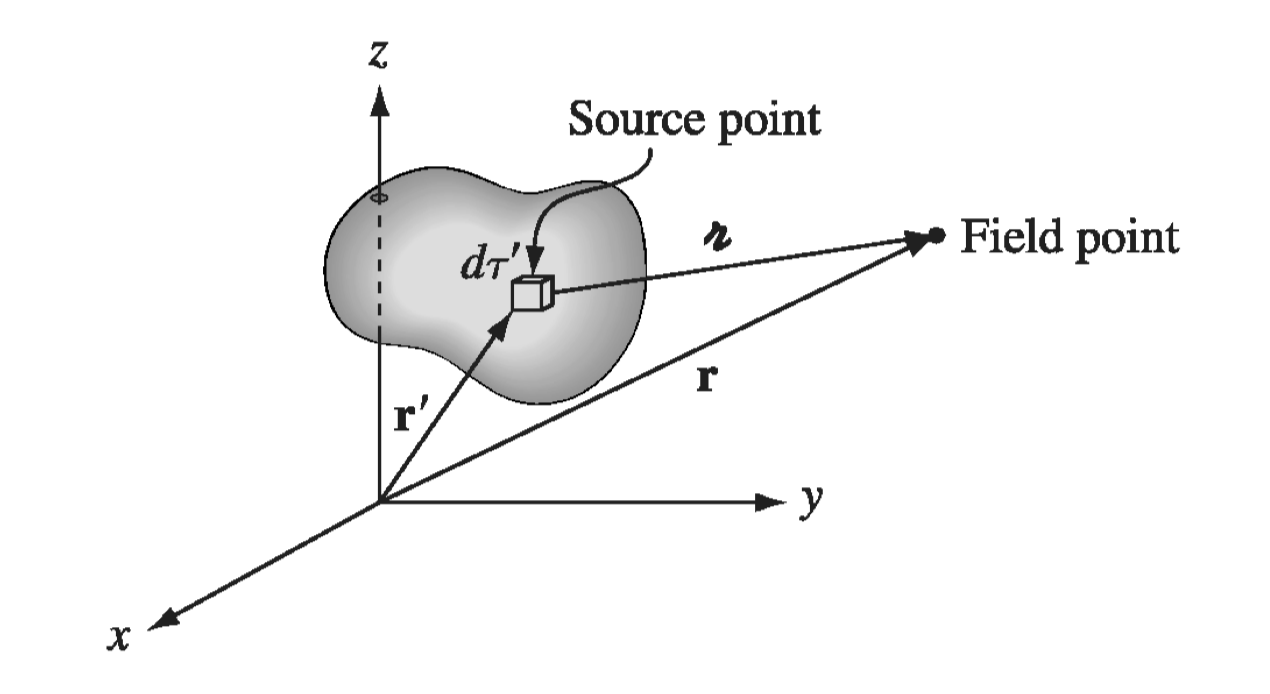
\includegraphics[width = 0.6 \textwidth]{figure/Chapter1/notation.png}
\end{figure}






\chapter{Electrostatics}

\section{Basics}
\begin{figure}[h]
    \centering
    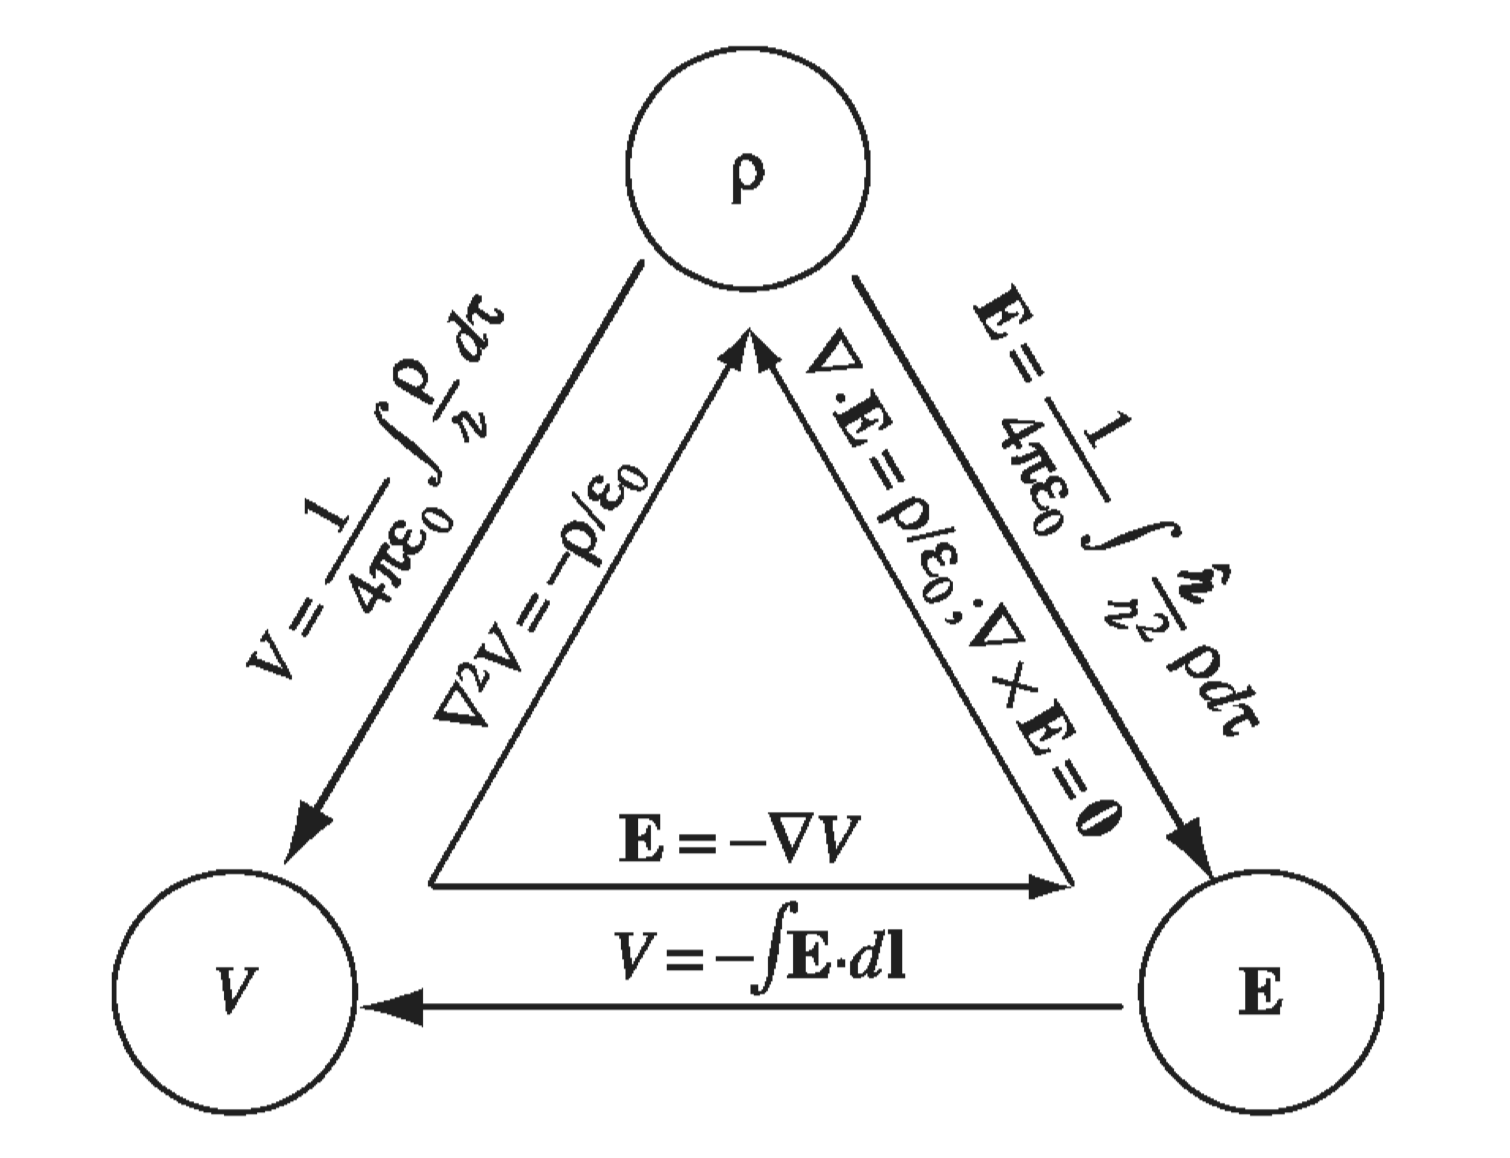
\includegraphics[width = 0.6 \textwidth]{figure/E_triangle_diagram.png}
    \caption{Triangle Diagram}
    \label{fig:E_triangle_diagram}
\end{figure}


\section{Boundary Conditions}

Across a surface charge (maybe the boundary of a conductor), the electric field is: 
\begin{equation}
    E = -\frac{\partial V}{\partial n} = \frac{\sigma}{\epsilon_0},
\end{equation}


\section{The Energy of Charge Distribution}

The amount of work it takes to assemble a configuration of charges; the amount of work you would get back if you dismantled the system. 
\begin{equation}
    W = \frac{1}{2}\sum_{i=1}^n q_i V(\mathbf{r_i}) = \frac{1}{2} \int \rho V d \tau = \frac{\epsilon_0}{2} \int E^2 d \tau. 
\end{equation}


\section{Conductors}
\subsection{Basics}
\begin{enumerate}
    \item \textbf{E = 0 inside a conductor} Because other wise charges will move. 
    \item $\mathbf{\rho = 0}$ \textbf{\fbox{\parbox{2.4em}{inside}} a conductor. }
    \item Any net charge resides on the surface
    \item A conductor is equipotential (both on the surface and inside).
    \item \textbf{E is perpendicular to the surface, just outside of the conductor. }
\end{enumerate}

The conductor behaves like a empty equipotential shell, see example 3.6 and 3.7. 


\chapter{Special Techniques for Solving Laplace Equation}
\section{Laplace's Equation}
\subsection{Uniqueness theorems}
\textbf{First uniqueness theorem}: The solution to Laplace's equation in some volume $\mathcal{V}$ is uniquely determined if $V$ is specified on the boundary surface $\mathcal{S}$. 

\textbf{Second uniqueness theorem}: In a volume $\mathcal{V}$ surrounded by conductors and containing a specified charge density $\rho$, the electric field is uniquely determined if the total charge on each conductor is given. 

\section{The Method of Images}
The key of the method is to use uniqueness theorems by finding another easier configuration with the same boundary conditions and satisfies the same Poisson's equation. 

\section{Separation of Variables}
\section{General Strategy}
\begin{enumerate}
    \item Make sure we are actually solving the Laplace's equation: we are trying to find potential where there is no charge distribution. 
    \item Find out what coordinates the Laplace's equation is dependent on and write down the Laplace's equation. General form for Cartesian coordinates: 
    \begin{equation}
        \frac{\partial^2 V}{\partial x^2}  + \frac{\partial^2 V}{\partial y^2} + \frac{\partial^2 V}{\partial z^2} = 0,
    \end{equation}
    spherical coordinates: 
    \begin{equation}
        \frac{1}{r^2} \frac{\partial}{\partial r} \left( r^2 \frac{\partial V}{\partial r}\right) + \frac{1}{r^2 \sin{\theta}} \frac{\partial}{\partial \theta} \left( \sin{\theta} \frac{\partial V}{\partial \theta} \right) + \frac{1}{r^2 \sin^2{\theta}}\frac{\partial^2 V}{\partial \phi^2} = 0
    \end{equation}
    
    \item Separate the variables, for Cartesian coordinates: 
    \begin{equation}
        V(x,y,z) = X(x)Y(y)Z(z);
    \end{equation}
    Spherical coordinates: 
    \begin{equation}
        V(r,\theta) = R(r)\Theta(\theta).
    \end{equation}
    
    \item Turn partial differential equation into ordinary ones, Cartesian Coordinate: 
    \begin{equation}
        \frac{d^2X}{dx^2} = C_1 X = (k^2 + l^2)X, \frac{d^2Y}{dy^2} = C_2 X = -k^2 Y, \frac{d^2Z}{dz^2} = C_3 X = -l^2 Z.
    \end{equation}
    Spherical Coordinates: 
    \begin{equation}
    \frac{d}{dr}\left( r^2 \frac{dR}{dr}\right) = l(l+1)R, \frac{d}{d\theta}\left(\sin{\theta} \frac{d\Theta}{d\theta}\right) = -l(l+1)\sin{\theta}\Theta.
    \end{equation}
    
    \item Solve them:
    \begin{align}
        X(x) &= Ae^{\sqrt{k^2 + l^2}x} + B e^{-\sqrt{k^2 + l^2}x}\\
        Y(y) &= C\sin{ky} + D\cos{ky},\\
        Z(z) &= E\sin{lz} + F\cos{lz}. 
    \end{align}
    And, 
    \begin{align}
        R(r) &= A r^l + \frac{B}{r^{l+1}}\\
        \Theta(\theta) &= P_l(\cos{\theta}).
    \end{align}
    $P_l(x)$, Legendre polynomials, are defined by \textbf{Rodrigues formula}: 
    \begin{equation}
        P_l(x) = \frac{1}{2^l l!} \left( \frac{d}{dx}\right)^l (x^2 - 1)^l.
    \end{equation}
    
    
    \item Take linear combination of the general solutions: 
    
    \textbf{Spherical Coordinates}: 
    \begin{equation}
        V(r,\theta) = \sum_{l=0}^\infty \left( A_lr^l + \frac{B_l}{r^{l+1}} \right) P_l (\cos{\theta}). 
    \end{equation}
    
    \item Check for boundary condition at specified values and infinity to eliminate constants that blow up. 
    
    \item Using the fact that sines and Legendre polynomials are orthogonal function and apply Fourier's trick: 
    
    \textbf{Legendre Polynomial}: 
    \begin{align}
        \int_{-1}^1 P_l(x)P_{l'}(x)dx &= \int_0^{\pi} P_l(\cos{\theta})P_{l'}(\cos{\theta})\sin{\theta}d\theta\\
        & = 
        \begin{cases}
        \displaystyle 0, & \text{if\;} l' \neq l\\
        \displaystyle \frac{2}{2l+a}, & \text{if\;} l' = l.
        \end{cases}
    \end{align}
    So, we multiply the equation with the constant term and boundary condition, it may be $V_0(\theta)$ or calculated using formula from previous chapter: 
    \begin{equation}
        \text{Const.} \frac{2}{2l' + 1} = \int_0^{\pi} \text{boundary condition} \times P_{l'}(\cos{\theta})\sin{\theta}d\theta
    \end{equation}
\end{enumerate}

    
\subsection{Cartesian Coordinates Examples}
\begin{figure}[h]
    \centering
    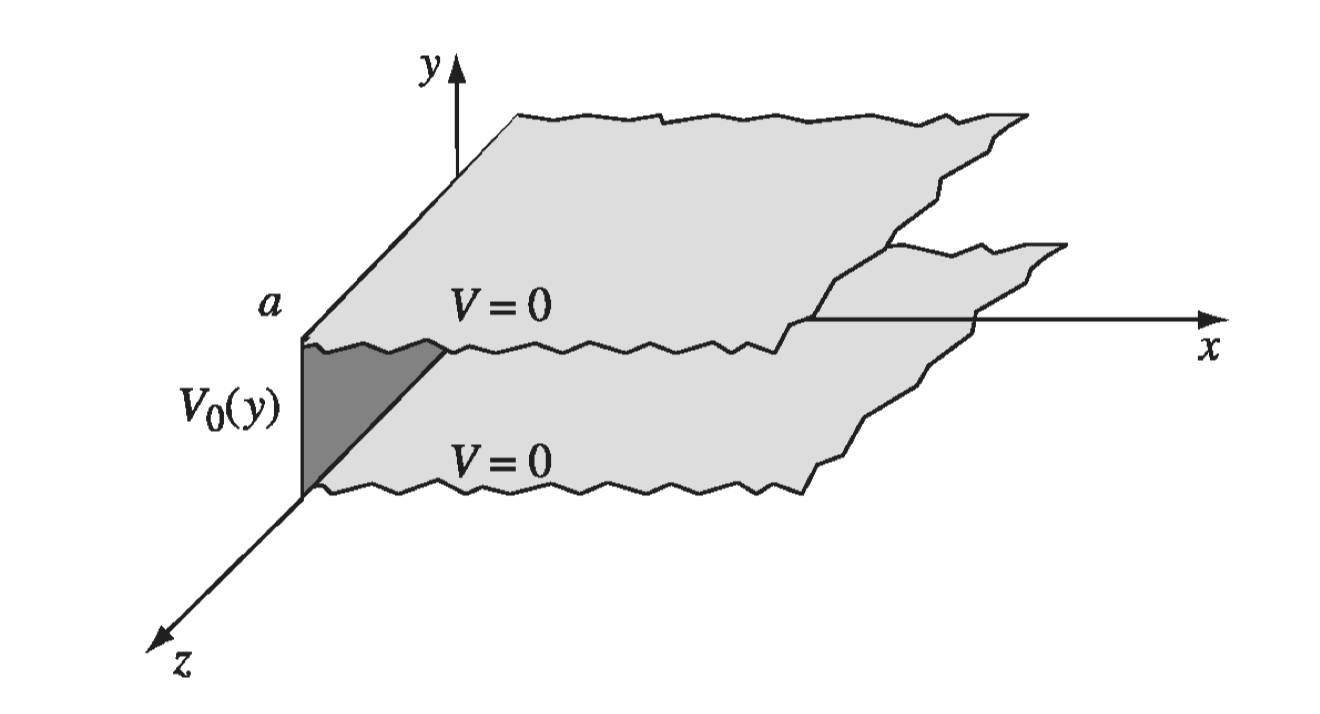
\includegraphics[width = 0.4 \textwidth]{figure/Chapter3/Ep3.3.png}
    \caption{Insulated two plates}
    \label{fig:ep3.3}
\end{figure}
General solution: 
\begin{equation}
    V(x,y) = \sum_{n=1}^\infty C_n e^{-n\pi x/a} \sin{(n\pi y/a)}
\end{equation}
To get coefficient $C_n$,
\begin{equation}
    V_0(y) = V(0,y) = \sum_{n=1}^\infty C_n \sin{(n\pi y/a)}.
\end{equation}
Apply \textbf{Fourier's trick}: multiply it by $\sin{n'\pi y/a}$ and integrate from 0 to $a$: 
\begin{equation}
    \int_0^a V(y) \sin{(n'\pi y/a)} dy = \sum_{n=1}^\infty C_n \int_0^a \sin{(n\pi y/a)}\sin{(n'\pi y/a)}dy.
\end{equation}
Now \begin{equation}
    \int_0^a \sin{(n\pi y/a)}\sin{(n'\pi y/a)} = \begin{cases}
      0, & \text{if\;} n' \neq n\\
      \frac{a}{2}, & \text{if\;} n = n'.
    \end{cases}
\end{equation}
So, dropping the dummy variable: \begin{equation}
    C_n = \frac{2}{a}\int_0^a V(y) \sin{(n'\pi y/a)} dy
\end{equation}


\section{Multiple Expansion}

\begin{figure}[h!]
    \centering
    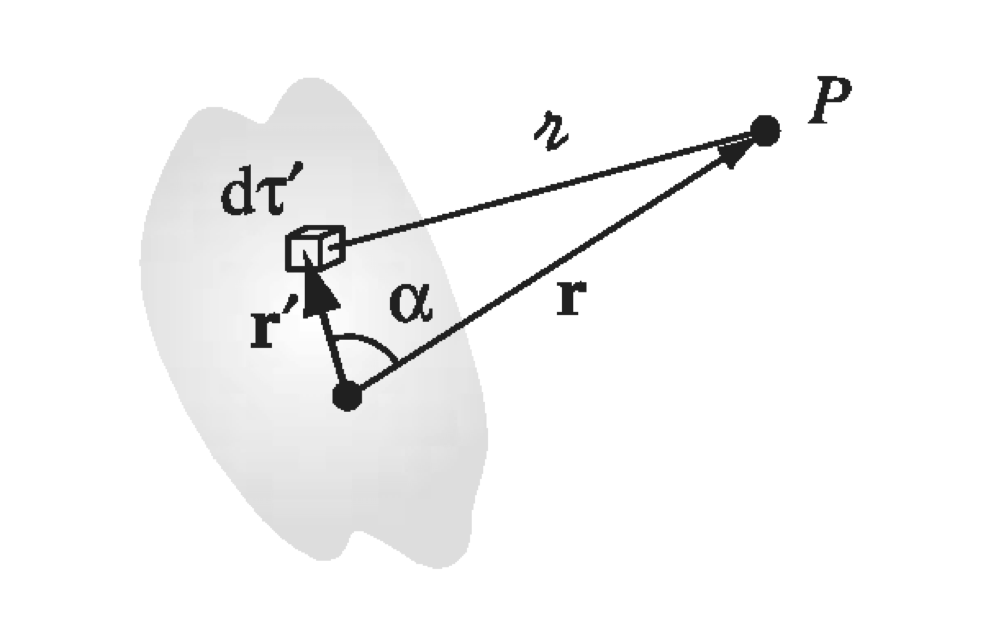
\includegraphics[width = 0.5 \textwidth]{figure/Chapter3/localized_charge_distribution.png}
    \caption{Caption}
    \label{fig:my_label}
\end{figure}
\begin{equation}
    V(\mathbf{r}) = \frac{1}{4 \pi \epsilon_0} \sum_{n = 0}^\infty \frac{1}{r^{(n+1)}} \int (r')^n P_n(\cos{\alpha})\rho(\mathbf{r}') d\tau'.
\end{equation}

\chapter{Magnetostatics}
\section{The divergence and curl of B}

\subsection{Amp\'ere's law}
There are four main prototype configurations where Amp\'ere's law is useful. 

\subsection{Special notes}
Often we can decide if a magnetic field has radial component by thinking about if reversing the direction of the flow of the current the direction of magnetic field changes. 


\end{document}
